In  this  section, we  present  a  performance  and energy  efficiency
evaluation  of  different  achitectures  when  running  the  COSMO-ART
baseline.  We  start by  specifying our measurement  methodology along
with the metrics used to  analyse the results on all platforms.  Then,
we detail the environment  setup gathering the considered HPC systems,
the software  environment and the runtime  configuration.  Finally, we
discuss  benchmark   results  and  power-performance   traces  of  the
application.

\subsection{Measurement methodology}
\label{subsec:4.1}
We  approach  the  assessment  of  the energy  footprint  and  overall
performance    of    COSMO-ART    with    two    important    metrics:
\textit{time-to-solution}       and       \textit{energy-to-solution}.
Time-to-Solution  refers   to  the  total  wall  clock   time  of  the
application execution time. Energy-to-solution is the amount of energy
spent  to achieve  results.  Energy  consumption of  CSCS  clusters is
assessed  by sampling  the instantaneous  peak power  during execution
which  is then  averaged  and multiplied  by  the time-to-solution  to
determine energy-to-solution.   Whenever possible, multiple production
runs of COSMO-ART were  performed to illustrate the reproducibility of
the baseline, and quantify  the significant uncertainties in the power
measurement, as dictated by the available technology.

\subsection{Environment setup}
\label{subsec:4.2}
While hardware  platforms mature  and are replaced,  we have  chosen a
state-of-the-art  Intel's  third-generation   Core  (aka  Ivy  Bridge)
processing platform (called ``Monch'')  for our power measurements, as
it  is slated  to stay  in service  without hardware  upgrade  for the
duration  of  the Exa2Green  project.   In  principle  at least,  this
architecture could be recreated or found in an identical configuration
beyond the lifetime of the project.  Given that the baseline benchmark
can be reproduced  within an expected variance, and  that the baseline
run configuration  can be used in  all future versions of  the code, a
fair comparison  will be made  between the baseline and  the milestone
versions   of    COSMO-ART.    In   this    study,   a   complementary
energy-to-solution  benchmarking  comparison  is  carried out  on  the
``Pilatus'' cluster based  on Intel's previous-generation Sandy Bridge
processors, conventional  in HPC  systems and known  to be  more power
consuming.

\subsubsection{Monch (CSCS - ETH Zurich)}
Monch, which is installed  at the Swiss National Supercomputing Center
(CSCS) of ETH Zurich, is  a 10 rack NEC-provided and dual-socket Intel
Ivy Bridge-EP based cluster, utilised from people that are part of the
Swiss    Platform   for    Advanced   Scientific    Computing   (PASC,
\url{http://www.pasc-ch.org/}). It is composed of 312 standard compute
nodes, 24 large-memory compute nodes and 24 huge-memory compute nodes.
Each standard  compute node comprises two Intel  Ivy Bridge-EP E5-2660
v2 ten-core processors operating at 2.2 GHz, themselves connected by a
high speed  InfiniBand network, based  on Mellanox SX6036  managed FDR
switches, with a  56 Gb/s speed.  Each core has  32 KB instruction and
32 KB data L1  caches and 256 KB of L2 cache. All  the 10 core share a
25 MB L3 cache and the platform has 32GB of DDR3 1600 MHz RAM. For our
energy-to-solution benchmark,  a full rack of Monch  constituted of 52
standard  compute   nodes  (monchc[029-080])  was   considered.

\subsubsection{Pilatus (CSCS - ETH Zurich)}
Pilatus,  which  is installed  at  the  Swiss National  Supercomputing
Center (CSCS)  of ETH Zurich,  is a dual-socket Intel  Sandy Bridge-EP
based cluster  used as Piz  Daint pre-post processing cluster.   It is
composed of 42 compute nodes  and has 2 high-speed interconnects based
on FDR:  the first is dedicated to  the MPI traffic and  the second to
the storage high speed traffic.  The 2 login nodes and the 42 computes
nodes  consists in  11  twin-pair Intel  E5-Series  DALCO r2264i4t  2U
scalable compute modules.  Each  module contains 4 compute nodes based
on two Intel Xeon E5-2670  eight-core processors operating at 2.6 GHz,
themselves  connected by  a high  speed InfiniBand  network,  based on
Mellanox SX6036 managed FDR switches,  with a 56 Gb/s speed. Each core
has 32 KB instruction and 32 KB data L1 caches and 256 KB of L2 cache.
All the  8 core share a  20 MB L3 cache  and the platform  has 64GB of
DDR3 1600 MHz  RAM. For our energy-to-solution benchmark,  a full rack
of Pilatus  constituted of 42 standard  compute nodes (pilatus[03-44])
was considered.

\subsubsection{Sofware environment}
INT2LM  and the  COSMO-ART model  are  implemented in  Fortran 90  for
distributed  memory  parallel  computers  using  the  Message  Passing
Interface (MPI)  and are purely  MPI-parallel.  The software  stack on
both many-core  platforms was  controlled using the  modules framework
which gives  an easy and  flexible mechanism to  access to all  of the
CSCS  provided compilers,  tools  and applications.   For our  initial
benchmarking,  we opted  for  the GNU  compiler  (gcc/4.8.1 on  Monch,
gcc/4.8.2 on Pilatus) with the -O3 compiler flag as it generally gives
a  good  level  of optimization  and  the  code  runs faster  in  this
configuration  than when  compiled with  the intel  compiler (14.0.1).
Besides, we installed the  MPICH2 implementation of MPI (mvapich2/1.9)
as  well  as  the  commonly  used HDF5  (1.8.12)  and  NetCDF  (4.3.1)
libraries in favor of the  traditional GRIB library for the management
of extremely  large and complex data collections.   All computes nodes
have    an   operating   system    based   on    GNU/Linux   featuring
``2.6.32-358.11.1.el6.x86\_64''  and  ``3.0.101-0.15-default'' kernels
for Monch and Pilatus respectively.

\subsubsection{Run configuration}
A snapshot of the code, which includes, at least conceptually, all the
information needed  to reproduce the  energy-to-solution benchmarks of
COSMO-ART, was produced and run on a 1040 cores using 20 MPI tasks per
node on  Monch and  on a  1344 cores using  16 MPI  tasks per  node on
Pilatus.   The  calculated  region  was mapped  to  the  participating
processors using  a 2D-partitioning strategy.   The distribution along
the  x and  y  coordinates  was defined  by  setting: $nprocx=40$  and
$nprocy=26$ for  Monch and $nprocx=28$ and $nprocy=24$  as $nprocx$ is
usually  kept  bigger  than  $nprocy$.   Besides as  this  version  of
COSMO-ART  doesn't  make  use   of  the  GRIB  library,  we  specified
$nprocio=0$ for  GRIB I/O.  Hyperthreading  is not considered  in this
study as previous  attempts of its use revealed that  it always led to
higher energy-to-solution.\\

\subsection{Experimental results}
\label{subsec:4.3}

\begin{figure}[htbf]
  \begin{center}
    \includegraphics[width=0.48\textwidth]{Figs/NRJ_benchmark_Monch.eps}
    \caption{Monch: Isola E1 Rack 2 Total Power}
    \label{fig:1}
  \end{center}
\end{figure}

\begin{figure}[htbf]
  \begin{center}
    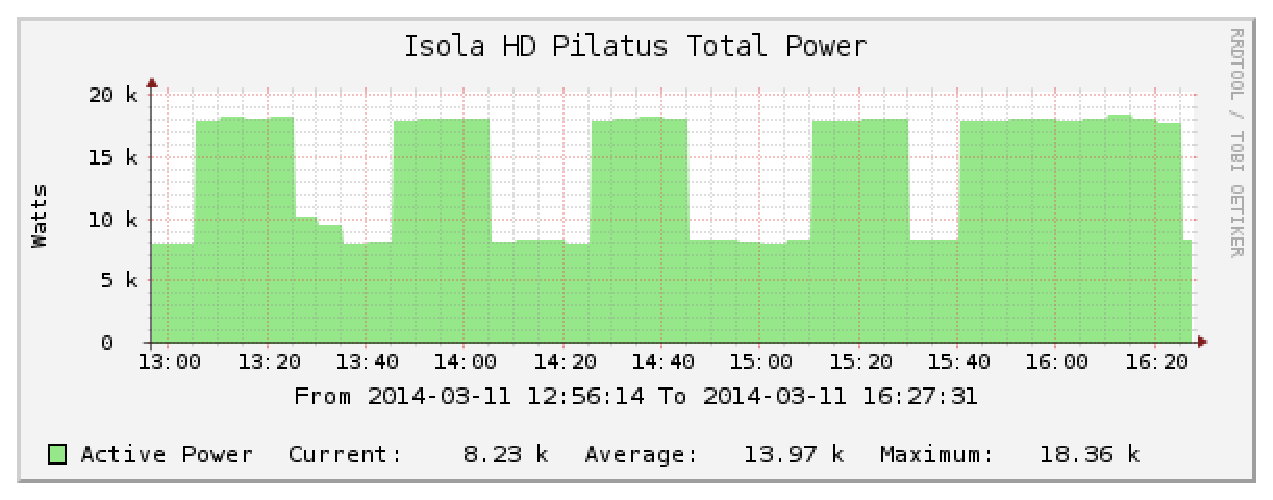
\includegraphics[width=0.48\textwidth]{Figs/NRJ_benchmark_Pilatus.eps}
    \caption{Pilatus: Isola HD Total Power}
    \label{fig:2}
  \end{center}
\end{figure}

Figures~\ref{fig:1} and  \ref{fig:2} account respectively  for Monch's
Isola E1  Rack 2  and Pilatus' Isola  HD total power  measurements for
1-day or 2-days simulations. On  the Intel Ivy Bridge EP based cluster
(i.e. Monch), the 1-day simulation  was issued only twice due to usage
restrictions. As time resolution was set to one update every 5 minutes
for  power sampling,  the average  power consumption  was  computed by
considering 6 values for each single  run.  On the Intel Xeon E5 based
cluster (i.e.   Pilatus), the 1-day  simulation was issued  four times
and a 2-days  run only once. Similarly, the  average power consumption
was computed by  considering 4 values for each single  1-day run and 9
values  for the  2-days  run. Corresponding  results  are gathered  in
Table~\ref{tab:3}.

\begin{table}[htbf]
  \begin{center}
    \caption{Average power consumption (W) of the platforms}
    \label{tab:3}
    \begin{tabular}{ccc}
      \hline\noalign{\smallskip}
      \textbf{Simulation time} & \textbf{Xeon E5} & \textbf{Ivy Bridge EP} \\
      \noalign{\smallskip}\hline\noalign{\smallskip}
      \textbf{1 day} & 18122.01417 & 12658.52278 \\ 
      & 17979.61083 & 12586.40833 \\
      & 18065.45167 & - \\
      & 17973.02833 & - \\
      \noalign{\smallskip}\hline\noalign{\smallskip}
      \textbf{2 days} & 17997.57815 & - \\
      \noalign{\smallskip}\hline
    \end{tabular}
  \end{center}
\end{table}

In Figure~\ref{fig:3}, we compare both time-to-solution (right y-axis)
and  energy-to-solution (left  y-axis) metrics  on both  platforms. As
expected,  Xeon  E5 outperforms  Ivy  Bridge  EP,  being roughly  1.3x
faster.  The reason for that is twofold: it has higher clock frequency
than Xeon E5 (2.6 GHz against  2.2 GHz) and it aims at computing speed
regardless to  energy consumption. In  our experiments, Ivy  Bridge EP
showed the best energy-to-solution, reducing the energy consumption of
Xeon E5 by approximately $7\%$.

\begin{figure}[htbf]
  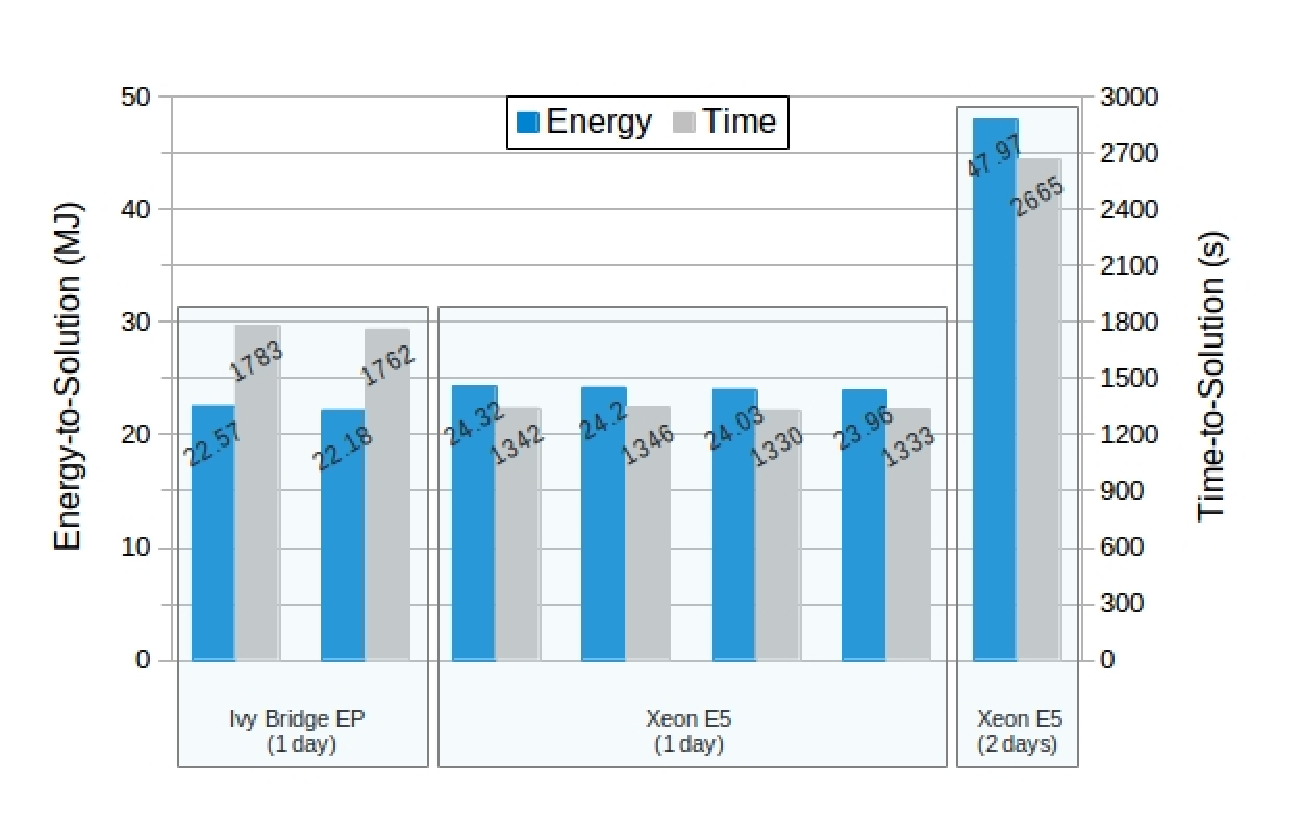
\includegraphics[width=0.5\textwidth]{Figs/Time_E2S_COSMO-ART.eps}
  \caption{Time-to-solution and  energy-to-solution comparison between
    Xeon E5 and Ivy Bridge-EP architectures}
  \label{fig:3}
\end{figure}


















